\section{Introduction}

\subsection{Overview}

The NUbots from the University of Newcastle, Australia have had a strong record of success in the RoboCup Four Legged League since first entering in 2002. The Nubots achieved 3rd place in 2002 (Fukuoka), and again in 2003 (Padua) and 2004 (Lisbon). In 2005 (Osaka) with a complete redevelopment of the code, the NUbots came 2nd in a heartbreaking penalty shoot out against the German Team. With a strong 2005 base code, 2006 development focused on debugging and fine tuning. The result was a nail biting final against rUNSWift in Bremen where the NUbots won 7-3. Code development plateaued in 2007 and we lost the final in Atlanta against the Northern Bites.  

2008 Involved the transition from the Sony ERS-7 robot to the Aldebaran Nao. We also created a joint team, The NUManoids with the the National University of Ireland, Maynooth (NUIM). Together we successfully overcame the challenges of adapting to the new hardware to become the first world champions of the Robocup Nao SPL.

For 2009 we separated from NUIM two create two independent teams and once again became the NUbots. We set out to improve the previous years code. The league as a whole made a great leap forward compared to the previous year. With major improvements to our vision, localisation and locomotion it was not enough to defend our title. We completed the competition with a ranking of quarter finalist.

This report will outline the system and some more recent advances added into the system for the 2009 RoboCup competition.

\subsection{Software Layout}

Our 2009 system was based on last years architecture \cite{NUManoids2008} which originated from the Sony Aibo architecture in 2006 \cite{NUBOT2006}. Our system consists of one control module \emph{Nao} and four functional modules -
\emph{Vision, Localisation, Behaviour and Locomotion}. 

The flow of information in our system can be seen in Figure
\ref{fig:software}. 

\begin{figure}[!ht]
\begin{center}
    %\leavevmode
    \scalebox{0.5} {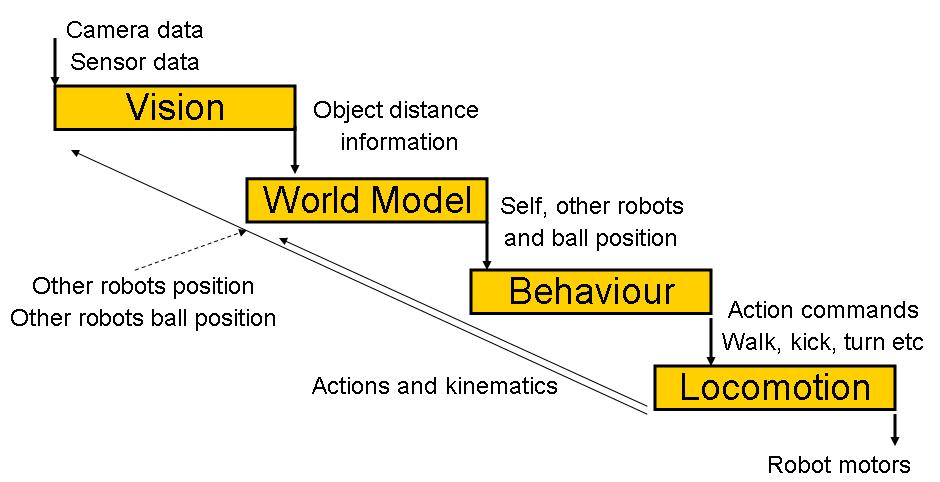
\includegraphics{figs/software.jpg} }
    \caption{2009 Software Architecture}
    \label{fig:software}
\end{center}
\end{figure}

